\documentclass[conference]{IEEEtran}
\IEEEoverridecommandlockouts
% The preceding line is only needed to identify funding in the first footnote. If that is unneeded, please comment it out.
\usepackage{cite}
\usepackage{amsmath,amssymb,amsfonts}
\usepackage{algorithmic}
\usepackage{graphicx}
\usepackage{textcomp}
\usepackage{xcolor}
\def\BibTeX{{\rm B\kern-.05em{\sc i\kern-.025em b}\kern-.08em
    T\kern-.1667em\lower.7ex\hbox{E}\kern-.125emX}}
\begin{document}

\title{Spectral-Guided Edge Blocking for Epidemic Containment in Directed Networks Using the SNIR Model\\

}

\author{\IEEEauthorblockN{1\textsuperscript{st} Lalith Chowdary }
\IEEEauthorblockA{\textit{Computer Science} \\
\textit{Shiv Nadar University}\\
vc239@snu.edu.in}
\and
\IEEEauthorblockN{2\textsuperscript{nd} Srinivas Tirumalaraju}
\IEEEauthorblockA{\textit{Computer Science} \\
\textit{Shiv Nadar University}\\
st437@snu.edu.in}
\and
\IEEEauthorblockN{3\textsuperscript{rd} Tanuj Kinjarapu}
\IEEEauthorblockA{\textit{Computer Science} \\
\textit{Shiv Nadar University}\\
tk641@snu.edi.in}
}

\maketitle

\begin{abstract}
To be written .....
\end{abstract}

\begin{IEEEkeywords}
To be written .....
\end{IEEEkeywords}

\section{Introduction}
Controlling the spread of epidemics and misinformation in social networks is a critical problem with real-world consequences in public health, cybersecurity, and online platforms. A central challenge in this domain is: given a limited intervention budget, which contacts in a network should be blocked to reduce the spread as much as possible? This is commonly known as the \textit{edge blocking} or \textit{contact isolation} problem.

Over the years, many methods have been proposed to tackle this problem, ranging from simple centrality-based heuristics to simulation-driven approaches and spectral graph theoretic methods. While each of these approaches has contributed meaningfully to the field, they each carry limitations --- either in accuracy, scalability, or their ability to handle directed networks realistically. These limitations are discussed in detail in Section~\ref{sec:related_work}.

In this paper, we propose a hybrid framework that combines two complementary approaches --- the SNIR epidemic simulation model and the spectral theory of directed networks --- to achieve more efficient and accurate edge blocking. The key idea is to use structural properties of the network to guide and reduce the search space before running expensive epidemic simulations, rather than evaluating every candidate edge blindly.

The main contributions of this paper are as follows:

\begin{itemize}
    \item \textbf{KSCC-based filtering:} We restrict candidate edges to the Key Strongly Connected Component (KSCC) of the directed network, which is the only region where edge removal can reduce the global spectral radius and thus the epidemic spread.
    
    \item \textbf{Spectral edge scoring:} We derive an $\mathcal{O}(1)$-per-edge approximation of the spectral radius reduction caused by edge removal, grounded in the Directed Chung-Lu spectral radius formula. For each edge $(u \to v)$ within the KSCC, we compute $\mathrm{SpectralDrop}(u{\to}v) \approx \rho(S^*) - \frac{\sum d_{\mathrm{in}} d_{\mathrm{out}} - d_{\mathrm{in}}^{S^*}(u) - d_{\mathrm{out}}^{S^*}(v)}{\mathrm{vol}(S^*)-1}$, converting node-level spectral theory from DINO into a principled edge-level ranking criterion.
    
    \item \textbf{Hybrid algorithm:} We integrate the above two steps into the SNIR framework to produce an algorithm that is faster than the original approach while maintaining the accuracy of epidemic-driven edge selection.
    
    \item \textbf{Empirical validation:} We evaluate our method on real-world directed networks and demonstrate its effectiveness and efficiency.
\end{itemize}


\section{Background}

This section provides the necessary background on the two frameworks that our method builds upon: the SNIR epidemic model with its edge blocking algorithm, and the spectral theory of directed networks from the DINO framework.

\subsection{The SNIR Epidemic Model}

The SNIR model proposed by Dai \textit{et al.} extends the classical SIR model by introducing a Non-symptomatic (N) state to capture asymptomatic infection, a pattern prominently observed in COVID-19. Every node in the network is in one of four states at any time: Susceptible (S), Non-symptomatic (N), Infectious (I), or Recovered (R).

Susceptible nodes can become asymptomatically infected with probability $\alpha$ or symptomatically infected with probability $\beta$. Non-symptomatic nodes spread the disease silently and may progress to Infectious with probability $\delta$ or recover directly with probability $\eta$. Infectious nodes recover with probability $\gamma$, and Recovered nodes may lose immunity and return to Susceptible with probability $\xi$.

The total expected infection over time horizon $T$ is measured as:
\begin{equation}
I(G, \Omega) = \sum_{t=0}^{T} \left[ \sum_{u \in V} P_N^W(u,t) + \sum_{u \in V} P_I^W(u,t) \right]
\end{equation}
where $\Omega = (S, N, I, R)$ is the initial network state and $W = N \cup I$ is the set of currently infectious nodes. The state probabilities at each time step are updated iteratively using a set of closed-form equations, avoiding the need for expensive Monte Carlo simulations.

\subsection{Extending SNIR to Directed Networks}

The original SNIR model was formulated and evaluated on undirected networks, where each edge $(u,v)$ represents symmetric contact and infection can flow in either direction. In a directed network, each edge $(u \to v)$ represents a one-way transmission channel. The existence of $(u \to v)$ does not imply $(v \to u)$, and the two carry independent transmission probabilities if both are present. Applying SNIR to directed networks requires modifying how the infection arrival probability is computed at each node.

In the undirected SNIR formulation, the probability that infection arrives at node $u$ at time $t{+}1$ aggregates contributions from all neighbors of $u$. In the directed setting, only nodes with a directed edge \emph{toward} $u$ can transmit to $u$. Formally, the directed transmission arrival probability is:
\begin{equation}
r(u,t{+}1) = 1 - \prod_{v:\,(v \to u) \in E} \bigl[1 - p(v,u) \cdot a(v,t)\bigr]
\end{equation}
where the product is taken only over nodes $v$ that have a directed edge to $u$, replacing the undirected neighborhood $\Gamma(u)$ with the directed in-neighborhood $N^{-}(u) = \{v \mid (v \to u) \in E\}$.

All subsequent SNIR state update equations for $p_I$, $p_N$, $p_R$, and $p_S$ remain structurally identical to the original formulation, updating as follows:
\begin{align}
p_I(u,t{+}1) &= (1-\gamma) p_I(u,t) + r(u,t{+}1) \beta p_S(u,t) + \delta p_N(u,t) \\
p_N(u,t{+}1) &= (1-\delta-\eta) p_N(u,t) + \alpha r(u,t{+}1) p_S(u,t) \\
p_R(u,t{+}1) &= (1-\xi) p_R(u,t) + \gamma p_I(u,t) + \eta p_N(u,t) \\
p_S(u,t{+}1) &= 1 - [p_N(u,t{+}1) + p_I(u,t{+}1) + p_R(u,t{+}1)]
\end{align}
The only modification propagates through $r(u,t{+}1)$, which now correctly reflects the asymmetric nature of directed contact. This extension ensures that a node can only receive infection through edges directed toward it, faithfully modeling directed transmission channels such as social media influence or physical flow networks. This directional specificity is what makes edge blocking on directed networks both more complex and more precise than on undirected networks.

\subsection{Edge Blocking Under the SNIR Model}

The edge blocking problem under the SNIR model is defined as follows: given a directed network $G = (V, E, P)$, an initial infected set, and a budget $k$, find at most $k$ edges whose removal minimizes $I(G, \Omega)$ over time $T$.

The MaxExpectedH algorithm of Dai \textit{et al.} solves this greedily. At each iteration, it identifies the candidate edge set:
\begin{equation}
\Gamma(W) = \{(u,v) \mid u \in W,\; v \notin W,\; (u,v) \in E \}
\end{equation}

For each candidate edge $e$, it computes:
\begin{equation}
H(e) = I(G_e, \Omega)
\end{equation}
by running a full SNIR simulation on the modified graph $G_e$. The edge with the smallest $H(e)$ is permanently removed, and the process repeats until $k$ edges are blocked.

While accurate, this approach is computationally expensive as it runs a full simulation for every candidate edge at every iteration.

\subsection{Spectral Theory of Directed Networks and DINO}

He \textit{et al.} established that epidemic spread on a directed network is governed by its spectral radius --- the largest eigenvalue magnitude of its adjacency matrix. Specifically, an epidemic dies out if and only if the spectral radius falls below a model-dependent threshold $C$.

They further proved a key structural result:

\textbf{Theorem:} The spectral radius of a directed network $G$ equals the spectral radius of its Key Strongly Connected Component (KSCC), defined as the strongly connected subgraph with the largest spectral radius.

This implies that interventions outside the KSCC have no effect on the global epidemic spread.

Additionally, under the Directed Chung-Lu network model, the spectral radius can be efficiently approximated as:
\begin{equation}
\rho(G) \approx \frac{\mathbf{d}^{in} \cdot \mathbf{d}^{out}}{\mathrm{vol}(G)}
\end{equation}
where $\mathbf{d}^{in}$ and $\mathbf{d}^{out}$ denote the in-degree and out-degree vectors, respectively, and $\mathrm{vol}(G)$ is the sum of all edge weights (or total degree in the unweighted case).

\subsection{The DINO Algorithm}

Based on the above theory, the DINO algorithm greedily removes $k$ nodes from the KSCC to maximally reduce the spectral radius. At each step, it selects the node $v$ minimizing the score function:
\begin{equation}
F(v) = \frac{\mathbf{d}^{in} \cdot \mathbf{d}^{out}}{\mathrm{vol}(G)}
\end{equation}
after removal, which approximates the spectral radius of the remaining graph.

Since $F(v)$ depends only on node degrees, the score for all nodes can be computed in linear time, giving DINO an overall complexity of $\mathcal{O}(k|V| + |E|)$.


\section{Research Gaps}

The previous section described two frameworks for epidemic containment --- the SNIR-based edge blocking approach and the DINO algorithm. While both are effective in their own way, they each have clear limitations. This section discusses these gaps and explains why a combined approach is needed.

\subsection{Computational Inefficiency of SNIR-Based Edge Blocking}

The MaxExpectedH algorithm produces accurate results by running a full SNIR simulation for every candidate edge at every iteration. While this yields high-quality results, it is computationally expensive.

The main issue is that the algorithm treats all candidate edges equally. It evaluates every edge in $\Gamma(W)$ with the same effort, regardless of whether the edge lies in a structurally critical region of the network or in a peripheral region with minimal influence on the spread. There is no mechanism to filter or prioritize edges before simulation. As the network size increases and the number of candidate edges grows, this exhaustive evaluation becomes a significant bottleneck.

\subsection{DINO Operates at the Wrong Granularity and Lacks Epidemic Realism}

DINO addresses the efficiency issue by leveraging spectral theory and a degree-based scoring function to select nodes in linear time. However, it has two key limitations in our setting.

First, DINO operates at the node level rather than the edge level. Removing a node effectively isolates an individual from all their contacts simultaneously, which is often impractical in real-world scenarios. In contrast, edge blocking --- restricting specific interactions --- is more realistic and actionable. For instance, during COVID-19, it was more feasible to restrict specific travel routes or interactions than to completely isolate individuals from all contacts.

Second, DINO lacks awareness of epidemic dynamics. Its scoring function depends only on node degrees and network structure, without considering factors such as current infection states, transmission probabilities, or temporal evolution of the epidemic. As a result, while DINO's selections may be structurally optimal, they may not correspond to the most effective interventions in a dynamic epidemic setting.

\subsection{Directed Networks Are Underexplored in Edge Blocking}

Most edge blocking methods, including MaxExpectedH, have been primarily designed and evaluated on undirected networks. Directed networks introduce additional complexity, as edges have directionality and transmission is not symmetric. Moreover, many spectral techniques developed for undirected graphs do not directly extend to the directed case.

The SNIR framework does not explicitly address the theoretical challenges of directed networks. On the other hand, DINO introduces important structural insights for directed graphs, such as the Key Strongly Connected Component (KSCC) and degree-based spectral approximations. However, these insights have not been applied to edge blocking problems, leaving a clear gap in the literature.

\subsection{Summary of Gaps}

In summary, SNIR-based methods provide accurate modeling of epidemic dynamics but suffer from inefficient exhaustive evaluation, while spectral methods such as DINO offer efficient structural guidance but lack support for edge-level interventions and realistic propagation dynamics.

An effective solution should combine the strengths of both approaches by:
\begin{itemize}
    \item focusing on structurally critical regions of the network,
    \item efficiently ranking candidate edges prior to evaluation, and
    \item incorporating realistic epidemic dynamics in the final decision process.
\end{itemize}

To the best of our knowledge, no existing method satisfies all these requirements simultaneously. This gap motivates the hybrid approach proposed in this work, which integrates spectral structural guidance with SNIR-based dynamic evaluation.


\section{Proposed Methodology: SG-SNIR}

This section presents the proposed algorithm, \textbf{SG-SNIR} (Spectral-Guided SNIR), a hybrid framework that integrates structural guidance from spectral graph theory into the SNIR epidemic simulation pipeline. The core idea is to reduce the expensive search space of SNIR-based edge blocking by first identifying structurally critical edges using KSCC analysis and bridge edge detection, and only then evaluating those edges through full epidemic simulation.

\subsection{Overview}

The algorithm operates in a greedy loop, selecting and removing one edge per iteration until the budget $k$ is exhausted. At each iteration, instead of evaluating all candidate edges with SNIR simulation, SG-SNIR first narrows the candidate set using two structural filters—KSCC membership and bridge edge detection—and then applies an adaptive spectral threshold to further reduce the set before simulation. The full flow of the algorithm is illustrated in Fig.~\ref{fig:sgsnir_flow}.

\begin{figure}[htbp]
\centering
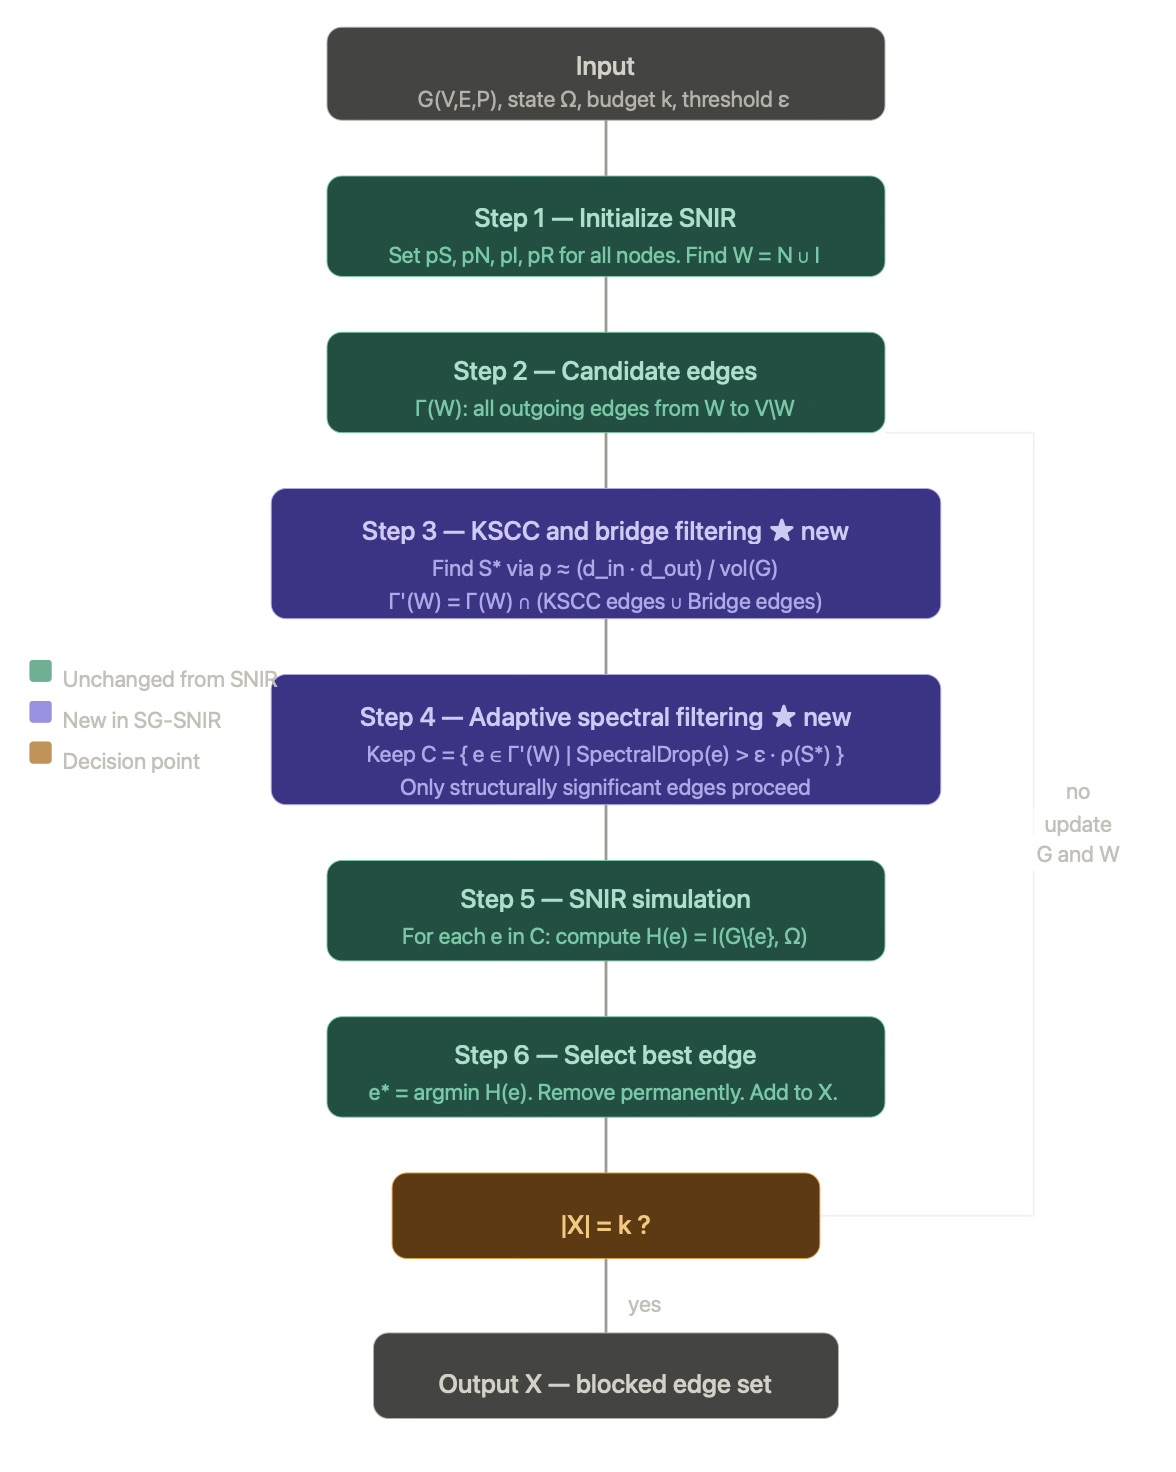
\includegraphics[width=0.9\linewidth]{sg_snir_flow.jpeg}
\caption{Overall workflow of the SG-SNIR algorithm.}
\label{fig:sgsnir_flow}
\end{figure}

\subsection{Step-by-Step Description}

\textbf{Step 1 — Initialize SNIR:}  
Given the initial network state $\Omega = (S, N, I, R)$, each node is assigned initial state probabilities $p_S, p_N, p_I, p_R$. The current infection source set is defined as:
\begin{equation}
W = N \cup I
\end{equation}
containing all nodes capable of spreading the disease.

\vspace{0.5em}

\textbf{Step 2 — Compute candidate edges:}  
The candidate edge set contains all outgoing edges from infectious nodes to \emph{Susceptible} nodes only:
\begin{equation}
\Gamma(W) = \{(u,v) \mid u \in W,\ v \in S,\ (u,v) \in E\}
\end{equation}
This is a refinement of the original MaxExpectedH candidate set, which used $v \notin W$. Here we further restrict to $v \in S$ since edges to Recovered nodes carry zero transmission probability under the SNIR model; blocking such edges provides no reduction in epidemic spread and wastes simulation budget.

\vspace{0.5em}

\textbf{Step 3 — KSCC and bridge filtering:}  
The algorithm decomposes the current graph into Strongly Connected Components (SCCs) using Tarjan's algorithm. Trivial SCCs (single nodes with no self-loop) are discarded, as they have spectral radius zero and cannot sustain epidemic spread. For each remaining non-trivial SCC $S_i$, the spectral radius is approximated using only the \emph{intra-SCC} degrees:
\begin{equation}
\rho(S_i) \approx \frac{\displaystyle\sum_{u \in S_i} d_{\mathrm{in}}^{S_i}(u)\, d_{\mathrm{out}}^{S_i}(u)}{\mathrm{vol}(S_i)}
\end{equation}
where $d_{\mathrm{in}}^{S_i}(u)$ counts only edges whose both endpoints lie within $S_i$, and $\mathrm{vol}(S_i) = \sum_{u \in S_i} d_{\mathrm{in}}^{S_i}(u)$. The Key Strongly Connected Component is then identified as:
\begin{equation}
S^* = \arg\max_{S_i} \; \rho(S_i)
\end{equation}

\textit{Note:} using full-graph degrees would conflate the structural properties of different SCCs and produce an incorrect identification of the KSCC.

The filtered candidate set is then defined as:
\begin{equation}
\Gamma'(W) = \Gamma(W) \cap \left(\mathcal{E}_{S^*} \cup \mathcal{B}_{S^*}\right)
\end{equation}
where $\mathcal{E}_{S^*}$ is the set of edges internal to $S^*$, and $\mathcal{B}_{S^*}$ is the set of bridge edges into $S^*$. A bridge edge is any edge $(u \to v)$ where $u \notin S^*$ and $v \in S^*$, representing infection entry points into the highest-spread region of the network.

If $\Gamma'(W) = \emptyset$ but $\Gamma(W) \neq \emptyset$, the current epidemic is confined to a region disconnected from the KSCC. In this case structural filtering is bypassed and $\Gamma'(W) = \Gamma(W)$, ensuring the algorithm always makes progress on locally active outbreaks.

\vspace{0.5em}

\textbf{Step 4 — Adaptive spectral filtering:}  
For each internal KSCC edge $(u \to v) \in \mathcal{E}_{S^*}$, we define $\mathrm{SpectralDrop}$ as the estimated reduction in $\rho(S^*)$ from permanently removing that edge:
\begin{equation}
\mathrm{SpectralDrop}(u{\to}v) = \rho(S^*) - \rho(S^* \setminus \{u{\to}v\})
\end{equation}
Computing this exactly requires a full spectral recomputation. Instead, we use the Directed Chung-Lu approximation. When $(u \to v)$ is removed from $S^*$, $d_{\mathrm{out}}^{S^*}(u)$ decreases by 1 and $d_{\mathrm{in}}^{S^*}(v)$ decreases by 1. The consequent change in the degree-product sum $\sum d_{\mathrm{in}} d_{\mathrm{out}}$ is derived as:
\begin{align*}
\Delta \text{sum} &= \bigl[ d_{\mathrm{in}}(u) d_{\mathrm{out}}(u) - d_{\mathrm{in}}(u) (d_{\mathrm{out}}(u)-1) \bigr] \\
&\quad + \bigl[ d_{\mathrm{in}}(v) d_{\mathrm{out}}(v) - (d_{\mathrm{in}}(v)-1) d_{\mathrm{out}}(v) \bigr] \\
&= d_{\mathrm{in}}(u) + d_{\mathrm{out}}(v)
\end{align*}
reducing the overall numerator sum by $d_{\mathrm{in}}^{S^*}(u) + d_{\mathrm{out}}^{S^*}(v)$. This gives the $\mathcal{O}(1)$-per-edge approximation:
\begin{equation}
\mathrm{SpectralDrop}(u{\to}v) \approx \rho(S^*) - \frac{\displaystyle\sum_{i \in S^*} d_{\mathrm{in}}^{S^*}(i)\,d_{\mathrm{out}}^{S^*}(i) - d_{\mathrm{in}}^{S^*}(u) - d_{\mathrm{out}}^{S^*}(v)}{\mathrm{vol}(S^*) - 1}
\end{equation}
Note that Equation 17 is defined only for edges $(u \to v)$ where both $u$ and $v$ lie within $S^*$. Bridge edges are handled separately as described in Equation 18. Since the numerator sum and $\mathrm{vol}(S^*)$ are precomputed once per iteration, $\mathrm{SpectralDrop}$ for all internal edges in $\Gamma'(W)$ is evaluated in $\mathcal{O}(|\Gamma'(W)|)$ total time.

The adaptive candidate set is constructed with bimodal filtering. Bridge edges bypass the spectral threshold entirely. Bridge edges have $\mathrm{SpectralDrop} = 0$ because their source node $u$ lies outside $S^*$, meaning neither $d_{\mathrm{in}}^{S^*}(u)$ nor $d_{\mathrm{out}}^{S^*}(u)$ appear in the KSCC degree-product sum. Removing such an edge does not alter any intra-KSCC degree, leaving $\rho(S^*)$ unchanged under the Chung-Lu approximation. Their importance is epidemiological rather than spectral — they represent the only pathways through which infection can enter $S^*$ from outside, and blocking them prevents the KSCC from being seeded entirely:
\begin{equation}
C = \mathcal{B}_{S^*}^{\Gamma} \;\cup\; \{e \in \mathcal{E}_{S^*}^{\Gamma} \mid \mathrm{SpectralDrop}(e) > \varepsilon \cdot \rho(S^*)\}
\end{equation}
where $\mathcal{B}_{S^*}^{\Gamma} = \Gamma'(W) \cap \mathcal{B}_{S^*}$ and $\mathcal{E}_{S^*}^{\Gamma} = \Gamma'(W) \cap \mathcal{E}_{S^*}$.

If $C = \emptyset$ after this filtering step, the spectral threshold is relaxed and $C = \Gamma'(W)$, guaranteeing the algorithm always selects an edge and fully expends the budget $k$.

\vspace{0.5em}

\textbf{Step 5 — SNIR simulation:}  
For each edge $e \in C$, the algorithm temporarily removes $e$, runs the full SNIR propagation for $T$ time steps, and computes:
\begin{equation}
H(e) = I(G_e, \Omega)
\end{equation}

\vspace{0.5em}

\textbf{Step 6 — Select and remove best edge:}  
\begin{equation}
e^* = \arg\min_{e \in C} H(e)
\end{equation}

This edge is permanently removed from $G$ and added to the selected set $X$. The algorithm returns to Step 2 with the updated graph. The infected set $W$ is held fixed throughout all $k$ iterations — the algorithm operates as a \emph{static budget allocation}, identifying and removing all $k$ edges prospectively from the initial configuration at $t=0$. This models a realistic, immediate intervention scenario (e.g., ``Day 1'' of an outbreak) where the entire intervention budget must be deployed simultaneously to preemptively halt the spread, rather than allocating interventions dynamically as the epidemic evolves in the future. A limitation of this static approach is that if an epidemic has already been spreading dynamically for some time, the upfront fixed $W$ may eventually miss critical emergent transmission pathways. Expanding the algorithm to support dynamic recalculation of $W$ remains an area for future work. The process repeats until $|X| = k$ or $\Gamma(W) = \emptyset$.



\section{Datasets}

To be written ....
\section{Evaluation metrics}

To be Written .....

\section*{Results and Conclusions}

To be written .....

\section*{References}

To be written .....

\end{document}
